\section{Many electrons and density-functional theory}\label{sec:3.4}

A density-functional calculation of silicon, the source of the bands behind computed dark-matter rates, puts the gap at about \SI{0.5}{eV}, less than half the measured \SI{1.17}{eV}. Density-functional theory computes the potential $U(\vect{r})$ of \cref{sec:3.2} from the electrons themselves instead of fitting it, and the gap is its best-known failure. Since the threshold mass of \cref{eq:1.3-mmin} is proportional to the gap, the error enters the reach directly: the computed gap would put the reach of a silicon detector at \SI{0.15}{MeV} instead of \SI{0.33}{MeV}. The many-electron problem of \cref{eq:2.3-HC} can be reduced to one electron in an effective potential, first by the best single Slater determinant and then by the Kohn--Sham construction. The eigenvalues that come out are not the energies to add or remove an electron, and the standard repair, a rigid shift of the conduction bands, changes the energies and some of the matrix elements of a rate.

\subsection{Hartree--Fock theory}

The simplest many-electron state with the right antisymmetry is a single Slater determinant $|\Phi_0\rangle$, \cref{eq:2.3-slater}, built from $N_e$ orthonormal orbitals $\psi_\gamma(x)$, with $x = (\vect{r}, s)$ the position and spin. Its Coulomb energy is a direct (Hartree) term minus an exchange (Fock) term (\cref{sec:2.3}). By the variational principle the energy of any state is at least the exact ground-state energy $E_0$, so the best determinant is the one of lowest energy. The orbitals are varied under the constraint that they stay orthonormal. The minimum condition is the set of \emph{Hartree--Fock equations} (\cref{app:D.4}):
\begin{equation}
  \Bigl[-\frac{\nabla^2}{2m_e} + U_1(\vect{r}) + v_{\mathrm{H}}(\vect{r})\Bigr]\psi_\gamma(x) + \int\dd x'\,\Sigma_{\mathrm{x}}(x, x')\,\psi_\gamma(x') = E_\gamma\,\psi_\gamma(x) .
  \label{eq:3.4-HF}
\end{equation}
Here $U_1$ is the attraction of the clamped nuclei, $v_{\mathrm{H}}(\vect{r}) = \int\dd^3r'\,e^2\nd(\vect{r}')/4\pi|\vect{r} - \vect{r}'|$ is the electrostatic potential of the electron density $\nd(\vect{r})$, and the exchange term
\begin{equation*}
  \Sigma_{\mathrm{x}}(x, x') = -\frac{e^2}{4\pi|\vect{r} - \vect{r}'|}\sum_{\gamma'\,\mathrm{occ}}\psi_{\gamma'}(x)\psi^*_{\gamma'}(x') ,
\end{equation*}
couples each electron only to occupied orbitals of the same spin. The equations are nonlinear, since the potentials are built from the occupied solutions, and they are iterated until the orbitals that go in are the ones that come out. This is the \emph{self-consistent field}. The orbitals of the atoms behind the ionization form factors of \cref{sec:2.2} are of this kind.

Each term has a plain meaning. The Hartree potential treats the other electrons as a smooth charge cloud. On its own it would also let each electron repel its own charge. The exchange term removes that self-repulsion exactly. Around every electron it digs a hole in the density of the electrons of the same spin, the exchange hole, which integrates to one missing electron. The exchange term is, however, an integral operator, not a function of $\vect{r}$. It acts on $\psi_\gamma$ through its values everywhere, and it is the first example in the book of a nonlocal one-electron operator, with the consequences for the velocity and the $f$-sum rule that \cref{sec:4.3} works out.

The eigenvalues $E_\gamma$ have a precise meaning, \emph{Koopmans' theorem}~\cite{koopmans1934zuordnung}. If the other orbitals are held fixed, $-E_\gamma$ is the energy needed to remove an electron from the occupied orbital $\gamma$, and the eigenvalue $E_\gamma$ of an empty orbital is the change in energy when an electron is added to it (\cref{eq:D.4-koopmans}). In a crystal the frozen-orbital hypothesis costs nothing. A Bloch state is spread over all $N$ cells, and removing it changes the density in each cell by a relative amount of order $1/N$. Since the energy is stationary in the orbitals, letting them relax lowers it by a term of second order, which vanishes as $N \to \infty$ (\cref{app:D.4}). Hartree--Fock bands are therefore the removal and addition energies of the Hartree--Fock state, and their gap is its fundamental gap.

The trouble is that a single determinant has no correlation, and the electron gas shows how much that matters. There the Hartree--Fock bands can be computed in closed form, \cref{eq:D.4-gas}. At the valence density of silicon the exchange energy is \SI{-6.22}{eV} per electron, comparable to the kinetic energy of \SI{7.5}{eV} (\cref{eq:D.4-Ex}). Exchange widens the occupied band from the free \SI{12.5}{eV} to \SI{20.8}{eV}, and it makes the group velocity diverge logarithmically at the Fermi surface. Neither is seen in real metals. Both come from the long range of the bare exchange, $v_{\mathrm{C}}(k) \propto 1/k^2$, which in a real solid the other electrons screen. In a semiconductor the same unscreened exchange makes the Hartree--Fock gap far too large. An added electron is not allowed to push the others away, and a removed one does not let them close in, so both the addition and the removal energies come out too high in magnitude. We return to this picture when we compare gaps below.

\subsection{Density-functional theory}

The electron density of silicon is a function of three variables, while its ground-state wavefunction depends on the $3N_e$ coordinates of all the electrons. Hohenberg and Kohn showed that the density is enough~\cite{hohenberg1964inhomogeneous}. Their first theorem states that the ground-state density $\nd(\vect{r})$ determines the external potential $U_1$ up to a constant. With it, $\nd$ fixes the Hamiltonian and every property of the system, excited states included. Their second theorem turns this into a variational principle. In the constrained-search form of Levy~\cite{levy1979universal}, define the universal functional
\begin{equation*}
  \mathcal{F}[\nd] = \min_{\Psi\to\nd}\langle\Psi|H_{\mathrm{kin}} + H_{ee}|\Psi\rangle ,
\end{equation*}
the lowest kinetic plus Coulomb energy of any state of $N_e$ electrons with density $\nd$. It does not depend on the nuclei and is the same for silicon, germanium and a single atom. The ground-state energy in the potential $U_1$ is then the minimum over densities,
\begin{equation}
  E_0 = \min_{\nd}\Bigl(\mathcal{F}[\nd] + \int\dd^3r\,U_1(\vect{r})\,\nd(\vect{r})\Bigr),
  \label{eq:3.4-HK}
\end{equation}
reached at the ground-state density. \Cref{app:D.5} proves both statements. The proof of the first is a two-line contradiction between the variational principles of two Hamiltonians that would share a density; the second follows from doing the minimization over states in two steps, first at fixed density and then over densities. Neither says how to find $\mathcal{F}$.

Kohn and Sham made \cref{eq:3.4-HK} usable by computing the largest and hardest piece of $\mathcal{F}$ exactly~\cite{kohn1965self}. That piece is the kinetic energy. For independent electrons with the density $\nd$ it is $K_{\mathrm{s}}[\nd]$, the lowest kinetic energy of a single determinant with that density (written $T_{\mathrm{s}}$ in the literature). Together with the Hartree energy $E_{\mathrm{H}}[\nd]$, the classical electrostatic energy of the density, it leaves a remainder,
\begin{equation*}
  \mathcal{F}[\nd] = K_{\mathrm{s}}[\nd] + E_{\mathrm{H}}[\nd] + E_{\mathrm{xc}}[\nd] ,
\end{equation*}
which defines the \emph{exchange--correlation energy} $E_{\mathrm{xc}}$. It contains the exchange energy, which as in Hartree--Fock removes the self-repulsion in $E_{\mathrm{H}}$, the correlation energy that a determinant misses, and the part of the true kinetic energy that independent electrons do not have. It is the one piece that must be approximated. Minimizing over the orbitals of the determinant, as in \cref{app:D.4}, leads to one-electron equations.
\begin{keyresult}[Kohn--Sham equations]
The ground-state density is $\nd(\vect{r}) = \sum_s\sum_{\gamma\,\mathrm{occ}}|\psi_\gamma(\vect{r}, s)|^2$, summed over the $N_e$ lowest solutions of
\begin{equation}
  \begin{gathered}
  \Bigl[-\frac{\nabla^2}{2m_e} + V_{\mathrm{KS}}(\vect{r})\Bigr]\psi_\gamma(x) = E_\gamma\,\psi_\gamma(x) , \\
  V_{\mathrm{KS}}(\vect{r}) = U_1(\vect{r}) + v_{\mathrm{H}}(\vect{r}) + v_{\mathrm{xc}}(\vect{r}) , \qquad
  v_{\mathrm{xc}}(\vect{r}) = \frac{\delta E_{\mathrm{xc}}}{\delta\nd(\vect{r})} .
  \end{gathered}
  \label{eq:3.4-KS}
\end{equation}
With the exact $E_{\mathrm{xc}}$, the density and the ground-state energy are exact. In a crystal $\gamma \to n\vect{k}$ and $E_\gamma \to \varepsilon_{n\vect{k}}$.
\end{keyresult}
\Cref{eq:3.4-KS} has the form of the Hartree--Fock equations \cref{eq:3.4-HF}, with one difference: the Kohn--Sham potential is a local function of $\vect{r}$, where the Fock term was an integral operator. It is the potential $U(\vect{r})$ of \cref{eq:3.2-He}. It is lattice-periodic, because the density is, and every result of \cref{sec:3.2,sec:3.3} applies to its Bloch states. Unlike the fitted potential of \cref{sec:3.3}, it is computed. The density that enters it is that of the bonds, not a sum of spherical atoms. Through $v_{\mathrm{H}}$ and $v_{\mathrm{xc}}$, the charge piled up between neighboring atoms gives $V_{\mathrm{KS}}$ a (222) component, which the basis structure factor removes from the nuclear part; the (200) component vanishes for any potential with the symmetry of the crystal (\cref{we:3-diamond}, \cref{app:C.17}).

The ground-state energy, unlike the eigenvalues, has a physical meaning, and it is \cref{eq:D.5-Etot}. Minimizing it with respect to the lattice constant, or the positions of the atoms, yields the equilibrium structure, and its second derivatives yield the force constants of the phonons (\cref{sec:5.2}). In the local-density approximation, introduced next, the computed lattice constant of silicon is \SI{5.401}{\angstrom}, \SI{0.5}{\percent} below the measured one (\cref{sec:3.1}).

\paragraph{Exchange--correlation functionals.}
The \emph{local-density approximation} (LDA) assumes that each small volume of the solid contributes the exchange--correlation energy of a uniform electron gas of the local density,
\begin{equation}
  E_{\mathrm{xc}}^{\mathrm{LDA}}[\nd] = \int\dd^3r\,\nd(\vect{r})\,\varepsilon_{\mathrm{xc}}\bigl(\nd(\vect{r})\bigr) ,
  \label{eq:3.4-LDA}
\end{equation}
with $\varepsilon_{\mathrm{xc}}(\nd)$ the energy per electron of the gas~\cite{kohn1965self}. Its exchange part is the Hartree--Fock result \cref{eq:D.4-Ex}, $\varepsilon_{\mathrm{x}} = -3e^2k_{\mathrm{F}}/16\pi^2$ with the local $k_{\mathrm{F}} = (3\pi^2\nd)^{1/3}$, and the exchange potential that follows is $v_{\mathrm{x}}^{\mathrm{LDA}} = \tfrac43\varepsilon_{\mathrm{x}}$, the Hartree--Fock exchange of an electron at the Fermi surface of the gas: \SI{-8.29}{eV} at the valence density of silicon (\cref{app:D.5}). The correlation part comes from quantum Monte Carlo energies of the gas~\cite{ceperley1980ground}, fitted as a function of the density~\cite{perdew1981self}. The approximation is exact for a uniform density and good when the density changes little over the local $1/k_{\mathrm{F}}$. Valence densities do not satisfy this, yet LDA works far better than the condition suggests, because the exchange--correlation hole it implies obeys the same sum rule as the exact one. The \emph{generalized-gradient approximations} (GGA) add a dependence on $|\nabla\nd|$; PBE~\cite{perdew1996generalized} is the one used most in solids. \emph{Hybrid functionals} replace part of the local exchange by the Fock term of \cref{eq:3.4-HF} built from the Kohn--Sham orbitals, which makes the potential nonlocal again; the hybrid functional of Heyd, Scuseria and Ernzerhof (HSE)~\cite{heyd2003hybrid} takes one quarter of the exchange from Fock, and only at short range. Each step from LDA to GGA to hybrids costs more, the hybrid step by one to three orders of magnitude (\cref{app:E.1}). Semilocal functionals give lattice constants within \SIrange{1}{2}{\percent}, LDA slightly too small and PBE slightly too large (\cref{tab:E-functionals}), and they give gaps that are much too small.

In practice, a Kohn--Sham calculation of silicon expands the periodic parts $u_{n\vect{k}}$ in plane waves, replaces the nuclei and core electrons by pseudopotentials (\cref{sec:3.5}), solves \cref{eq:3.4-KS} on a grid of crystal momenta, and iterates the density until it no longer changes (\cref{app:E.1}). The calculation of \cref{we:E-si-bands}, with the PBE functional and a norm-conserving silicon pseudopotential of the SG15 library (\cref{sec:3.5})~\cite{schlipf2015optimization}, takes seconds. At the measured lattice constant it places the conduction-band minimum at $k_{\mathrm{c}} = 0.843\,(2\pi/a)$ against the measured $0.85$, with a longitudinal valley mass $0.95\,m_e$ against $0.92\,m_e$ and a gap of \SI{0.557}{eV}, half the measured value (\cref{fig:3-si-bands}). Minimized in its total energy, the lattice constant comes out at \SI{5.477}{\angstrom}, \SI{0.85}{\percent} above the measured one, where the gap is \SI{0.602}{eV}. The electronic dielectric constant it computes is 13.04 against the measured 11.7 (\cref{sec:3.3}). The positions and curvatures of the bands are trustworthy; the gap is not, and the screening inherits part of its error.

\subsection{The band-gap problem}

A dark-matter threshold is an energy difference between many-electron states. The gap that a detector sees is the energy to take an electron out of the crystal at the top of the valence band and put it back at the bottom of the conduction band, far enough away that the two do not interact. With $E_{N_e}$ the ground-state energy of $N_e$ electrons, it is the \emph{fundamental gap}
\begin{equation}
  \Eg = \bigl(E_{N_e+1} - E_{N_e}\bigr) - \bigl(E_{N_e} - E_{N_e-1}\bigr) = I - A ,
  \label{eq:3.4-fundgap}
\end{equation}
the ionization energy $I$ minus the electron affinity $A$. More generally, the energy to add an electron in an empty state $n\vect{k}$, or minus the energy to remove one from an occupied state, is the \emph{quasiparticle energy} $E_{\mathrm{qp}}(n\vect{k})$, which \cref{sec:4.7} defines precisely as a pole of the one-electron Green's function. The bands that photoemission and inverse photoemission measure are quasiparticle bands, and the threshold of \cref{sec:3.3} is the difference of two of them.

The Kohn--Sham eigenvalues $\varepsilon_{n\vect{k}}$ are not quasiparticle energies. They are the Lagrange multipliers of a construction designed to reproduce the density, and only one of them has an exact meaning. By Janak's theorem~\cite{janak1978proof}, $\varepsilon_{n\vect{k}}$ is the derivative of the total energy with respect to the occupation of the state, and since the exact energy is a straight line between integer electron numbers~\cite{perdew1982density}, the highest occupied eigenvalue of the exact functional equals $-I$ (\cref{app:D.5}). The lowest empty eigenvalue would equal $-A$ only if the potential were the same on both sides of $N_e$. It is not. Since the exact energy is a straight line between integers, its slope, the chemical potential, jumps at $N_e$ from $-I$ to $-A$, by the fundamental gap. The slope of the Kohn--Sham kinetic energy $K_{\mathrm{s}}$ jumps only by the Kohn--Sham gap, because an added electron enters the lowest empty orbital. The Hartree energy is a smooth function of the density, so the rest of the jump must sit in $E_{\mathrm{xc}}$. When the electron number crosses $N_e$, the exact exchange--correlation potential jumps by a constant $\Delta_{\mathrm{xc}}$, the \emph{derivative discontinuity}, and even with the exact functional
\begin{equation}
  \Eg = E_{\mathrm{g}}^{\mathrm{KS}} + \Delta_{\mathrm{xc}} ,
  \label{eq:3.4-gap}
\end{equation}
with $E_{\mathrm{g}}^{\mathrm{KS}}$ the gap between the Kohn--Sham eigenvalues~\cite{perdew1983physical,sham1983density}. LDA and GGA are smooth functions of the density and have no discontinuity at all. For silicon, most of the difference between the LDA gap and the measured one is the missing $\Delta_{\mathrm{xc}}$, not an error of the LDA potential~\cite{godby1986accurate}. This is the \emph{band-gap problem}: the Kohn--Sham gap is too small for a reason that a better semilocal functional cannot remove.

LDA puts the silicon gap at \SI{0.52}{eV}, PBE at 0.56 to \SI{0.60}{eV}, against the measured \SI{1.17}{eV} (\cref{tab:E-gw,we:E-si-bands}). The error is similar in other semiconductors. GaAs comes out at \SI{0.43}{eV} in LDA against \SI{1.52}{eV}, and germanium, with a measured gap of \SI{0.744}{eV}, loses it: in LDA its gap closes (\cref{tab:E-functionals}), and in PBE with spin--orbit coupling its $s$-like conduction state at $\mathrm{\Gamma}$ falls below the valence-band maximum, which makes it a semimetal (\cref{fig:3-ge-gaas}). \Cref{fig:3-si-qp}(a) shows LDA bands of silicon. Their minimum gap, \SI{0.40}{eV} (lowered by about \SI{0.1}{eV} by the PBE-generated pseudopotential, see the caption), sits at $0.848\,(2\pi/a)$ along $\mathrm{\Gamma}$--$\mathrm{X}$, at the measured position, while quasiparticle energies and measured ones lie higher across the zone. In the figure, the $G_0W_0$ squares, from a separate calculation, sit 0.66 to \SI{0.70}{eV} above the solid LDA bands at the conduction states, and the dashed bands, shifted by one constant, pass close to all of them. The correction is not the same for every state, but within about \SI{0.1}{eV} the LDA conduction bands of silicon are right in shape and wrong in position.

\begin{figure}[tbp]
  \centering
  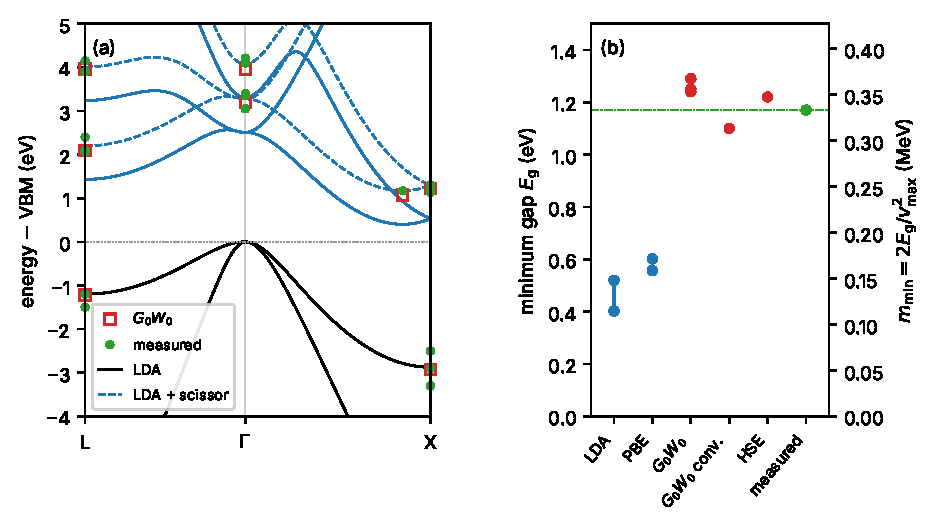
\includegraphics[width=\linewidth]{figures/ch03/fig3_8.pdf}
  \caption{The gap of silicon in density-functional theory, in quasiparticle calculations and in experiment. (a)~Solid: Kohn--Sham bands in the local-density approximation along $\mathrm{L}$--$\mathrm{\Gamma}$--$\mathrm{X}$, valence black and conduction blue, from the VBM; Slater exchange and Perdew--Zunger correlation~\cite{perdew1981self}, in the plane-wave calculation of \cref{app:E.1} (SG15 norm-conserving pseudopotential, \SI{60}{Ry}, $12^3$ grid, $a = \SI{5.431}{\angstrom}$, no spin--orbit coupling)~\cite{giannozzi2017advanced,hamann2013optimized,schlipf2015optimization}. Their minimum gap is \SI{0.40}{eV} at $0.848\,(2\pi/a)$; it changes by less than \SI{1}{meV} at \SI{80}{Ry} or on a $16^3$ grid, and the conduction states at $\mathrm{\Gamma}$, $\mathrm{X}$ and $\mathrm{L}$ lie at 2.51, 0.53 and \SI{1.43}{eV}. The pseudopotential was generated with PBE; a consistent LDA potential would raise the gap to about \SI{0.50}{eV}, close to the tabulated LDA value of \SI{0.52}{eV} (\cref{tab:E-gw}). Dashed: the same conduction bands shifted up by $\Delta_{\mathrm{scis}} = \SI{0.77}{eV}$, so that the minimum gap equals the measured \SI{1.17}{eV}. Squares: one-shot $G_0W_0$ quasiparticle energies, and circles: measured energies (all values listed there), both as given in Ref.~\cite[Tables~II and VI]{rideau2006strained}, at $\mathrm{\Gamma}$, $\mathrm{L}$, $\mathrm{X}$ and the conduction-band minimum. The $G_0W_0$ calculation is a different one from the LDA bands shown and includes spin--orbit coupling, whose splittings, below \SI{0.05}{eV}, are not resolved. (b)~Minimum gap from LDA~\cite[Table~I]{aryasetiawan1998gw} and from the LDA bands of panel (a), from PBE at the measured lattice constant (\cref{fig:3-si-bands}) and at the PBE lattice constant (\cref{we:E-si-bands}), from $G_0W_0$ calculations started from LDA~\cite{hybertsen1986electron,godby1988self,rohlfing1993quasiparticle} as collected in Ref.~\cite[Table~I]{aryasetiawan1998gw} and converged~\cite[Sect.~IV\,C]{klimes2014predictive}, from the hybrid functional HSE~\cite[Table~I]{lucero2012improved}, and measured at low temperature~\cite[Eq.~(11)]{ramanathan2020ionization}. Right axis: the threshold mass $m_{\mathrm{min}} = 2\Eg/v_{\mathrm{max}}^2$ of \cref{eq:1.3-mmin}, $v_{\mathrm{max}} = 2.650\times10^{-3}$.}
  \label{fig:3-si-qp}
\end{figure}

Why are quasiparticle gaps larger than Kohn--Sham gaps, and smaller than Hartree--Fock ones? A physical picture follows from what each theory lets the other electrons do, as anticipated above. In Hartree--Fock, an electron in an occupied state is bound by the exchange with the other electrons of its spin, while an electron in an empty state has no exchange with itself; this difference, of order the exchange energy of several eV, opens the gap. But the other electrons are frozen. A real added electron repels the electrons around it and polarizes the crystal, and the polarization lowers its energy; a real hole attracts them, with the same effect on the energy to create it. Both corrections close the gap. They come from screening, which at long range cuts the exchange interaction down by $1/\varepsilon_\infty$, a factor of 12 in silicon. The result is screened exchange: the exchange of Hartree--Fock with the bare Coulomb interaction replaced, at long range, by the interaction screened by $\varepsilon_\infty$, together with the energy of the polarization cloud that the particle carries along, the Coulomb-hole term of \cref{app:E.3}. A local Kohn--Sham potential is at the other extreme. It acts in the same way on occupied and empty states, and does not contain the discontinuity in the cost of adding an electron. The quasiparticle gap lies between the two limits, and in a strongly screening semiconductor it lies closer to the Kohn--Sham one. The $GW$ approximation of \cref{sec:4.8} makes this picture quantitative: its self-energy is the exchange with the dynamically screened interaction $W^{\mathrm{scr}}$. Started from LDA, it gives the silicon gap at 1.24 to \SI{1.29}{eV} in the calculations of the 1980s and early 1990s~\cite{hybertsen1986electron,godby1988self}\cite[Table~I]{aryasetiawan1998gw}, and at \SI{1.10}{eV} when converged with current methods~\cite[Sect.~IV\,C]{klimes2014predictive}. Hybrid functionals use the same idea crudely, with a fixed fraction of the Fock exchange; HSE gives \SI{1.22}{eV} (\cref{fig:3-si-qp}(b)).

The gap error reaches every quantity of a dark-matter rate that depends on energy differences across the gap. The threshold mass $m_{\mathrm{min}} = 2\Eg/v_{\mathrm{max}}^2$ is proportional to the gap, and the minimum pair energy $E_{\mathrm{min}}(\vect{q})$ of \cref{eq:3.3-Emin} moves with the conduction bands. Effective masses at a direct gap scale with it through \cref{eq:3.3-kane2}, as the Kane estimate of \cref{sec:3.3} shows for GaAs. The silicon valleys are less sensitive, since their mass comes from distant bands, and the PBE longitudinal mass is only \SI{4}{\percent} too heavy (\cref{app:E.1}). The screening is affected as well. Every transition contributes to $\varepsilon_\infty - 1$ more strongly the smaller its energy, and a gap that is too small makes the screening too strong, 13.04 against 11.7 in the PBE calculation of \cref{app:E.1}. The in-medium screening of \cref{chap:4} suppresses a rate by $|\varepsilon|^{-2}$, and it then suppresses it too much. A computed rate is therefore only as good as the gap behind it. Where the gap is measured, it can be imposed; where it is not, the spread of the methods in \cref{fig:3-si-qp}(b), about \SI{0.1}{eV} in silicon among calculations that treat the gap seriously, is a theory uncertainty of the threshold.

\subsection{The scissor shift}

Since the LDA or PBE conduction bands of silicon are nearly right in shape, the cheapest repair is to move them. The \emph{scissor shift} raises every conduction band by the same amount $\Delta_{\mathrm{scis}}$ and leaves the valence bands and all the states as they are:
\begin{equation}
  H^{\mathrm{s}}_{\vect{k}} = H_{\vect{k}} + \Delta_{\mathrm{scis}}\,P_{\mathrm{c}}(\vect{k}), \qquad
  P_{\mathrm{c}}(\vect{k}) = \sum_c|u_{c\vect{k}}\rangle\langle u_{c\vect{k}}| ,
  \label{eq:3.4-scissor}
\end{equation}
with $H_{\vect{k}}$ the Bloch Hamiltonian \cref{eq:3.2-Hk} of the Kohn--Sham potential and the sum over all conduction bands. Its eigenstates are those of $H_{\vect{k}}$, with eigenvalues $\varepsilon_{v\vect{k}}$ and $\varepsilon_{c\vect{k}} + \Delta_{\mathrm{scis}}$. The shift is chosen to bring the computed gap to a measured or a quasiparticle one: for the PBE calculation of \cref{we:E-si-bands}, $\Delta_{\mathrm{scis}} = 1.170 - 0.602 = \SI{0.568}{eV}$ at the PBE lattice constant, and \SI{0.613}{eV} at the measured one. Against full quasiparticle calculations, a rigid shift is good to about \SI{0.1}{eV} across the bands in silicon, and to 0.2 and \SI{0.4}{eV} in GaAs and diamond~\cite{godby1988self}\cite[Sect.~V\,B]{aryasetiawan1998gw}.

What does the shift do to the ingredients of a rate? Energies and the density vertex are easy. Every interband energy grows by $\Delta_{\mathrm{scis}}$, and so does $E_{\mathrm{min}}(\vect{q})$ at every $\vect{q}$. The density vertex $\rho_{cv}(\vect{k}, \vect{q})$ of \cref{eq:3.2-rho} is an overlap of states, and the states do not change. The velocity matrix elements are less obvious. $P_{\mathrm{c}}$ is a nonlocal operator, and the velocity, $\ii[H, \vect{r}]$, picks up a commutator with it. By \cref{eq:3.2-dHk}, the velocity matrix elements of $H^{\mathrm{s}}$ are those of $\nabla_{\vect{k}}H^{\mathrm{s}}_{\vect{k}}$. This operator contains the derivative of the projector,
\begin{equation*}
  \nabla_{\vect{k}}H^{\mathrm{s}}_{\vect{k}} = \nabla_{\vect{k}}H_{\vect{k}} + \Delta_{\mathrm{scis}}\sum_{c'}\Bigl(|\nabla_{\vect{k}}u_{c'\vect{k}}\rangle\langle u_{c'\vect{k}}| + |u_{c'\vect{k}}\rangle\langle\nabla_{\vect{k}}u_{c'\vect{k}}|\Bigr) .
\end{equation*}
Between a conduction state $c$ and a valence state $v$ at the same $\vect{k}$, the first term in the bracket contributes $\sum_{c'}\langle u_c|\nabla_{\vect{k}}u_{c'}\rangle\langle u_{c'}|u_v\rangle = 0$, since conduction and valence states are orthogonal. The second contributes $\langle\nabla_{\vect{k}}u_c|u_v\rangle$, the term $c' = c$ of $\sum_{c'}\langle u_c|u_{c'}\rangle\langle\nabla_{\vect{k}}u_{c'}|u_v\rangle$. Differentiating $\langle u_c|u_v\rangle = 0$ gives $\langle\nabla_{\vect{k}}u_c|u_v\rangle = -\langle u_c|\nabla_{\vect{k}}u_v\rangle$, and \cref{eq:3.2-dudk} gives $\langle u_c|\nabla_{\vect{k}}u_v\rangle = \vect{v}_{cv}/(\varepsilon_{v\vect{k}} - \varepsilon_{c\vect{k}})$. Altogether,
\begin{equation*}
  \vect{v}^{\mathrm{s}}_{cv}(\vect{k}) = \vect{v}_{cv}(\vect{k}) - \Delta_{\mathrm{scis}}\,\frac{\vect{v}_{cv}(\vect{k})}{\varepsilon_{v\vect{k}} - \varepsilon_{c\vect{k}}}
  = \vect{v}_{cv}(\vect{k})\Bigl(1 + \frac{\Delta_{\mathrm{scis}}}{\varepsilon_{c\vect{k}} - \varepsilon_{v\vect{k}}}\Bigr) .
\end{equation*}
Between two conduction states the two terms of the bracket give
\begin{equation*}
  \Delta_{\mathrm{scis}}\bigl(\langle u_c|\nabla_{\vect{k}}u_{c'}\rangle + \langle\nabla_{\vect{k}}u_c|u_{c'}\rangle\bigr) = \Delta_{\mathrm{scis}}\nabla_{\vect{k}}\langle u_c|u_{c'}\rangle = 0 ,
\end{equation*}
and between two valence states the projector does not act, so neither changes.
\begin{keyresult}[Scissor rescaling of the velocity]
Under the scissor shift \cref{eq:3.4-scissor}, energies and states transform as
\begin{equation}
  \begin{gathered}
  \varepsilon_{c\vect{k}} \to \varepsilon_{c\vect{k}} + \Delta_{\mathrm{scis}}, \qquad \rho_{mn}(\vect{k}, \vect{q}) \to \rho_{mn}(\vect{k}, \vect{q}), \\
  \vect{v}_{cv}(\vect{k}) \to \vect{v}_{cv}(\vect{k})\,\frac{\varepsilon_{c\vect{k}} - \varepsilon_{v\vect{k}} + \Delta_{\mathrm{scis}}}{\varepsilon_{c\vect{k}} - \varepsilon_{v\vect{k}}} ,
  \end{gathered}
  \label{eq:3.4-vscis}
\end{equation}
while the velocity matrix elements within the valence bands and within the conduction bands, the group velocities included, are unchanged.
\end{keyresult}
The interband velocity grows in proportion to the transition energy, and the optical limit \cref{eq:3.2-optical} shows why it must. The vertex $\rho_{cv} = \vect{q}\cdot\vect{v}_{cv}/(\varepsilon_{c\vect{k}} - \varepsilon_{v\vect{k}})$ is fixed because the states are fixed, so a larger denominator needs a larger numerator. The same follows from \cref{eq:3.2-r}: the position matrix element between the unchanged states stays the same, and the velocity is $\ii$ times the energy difference times it. \Cref{app:E.3} extends the rescaling to quasiparticle corrections that differ from state to state. At the direct gap of silicon at $\mathrm{\Gamma}$, \SI{2.55}{eV} in the PBE calculation at its own lattice constant, the shift of \SI{0.568}{eV} multiplies the velocity by $3.12/2.55 = 1.22$ and its square by 1.50. An absorption rate built from the shifted energies but the unshifted velocities comes out too small by that factor.

A scissor keeps the order of the Kohn--Sham bands, and where a functional gets that order wrong, as PBE does in germanium, whose conduction state at $\mathrm{\Gamma}$ falls below the $\mathrm{L}$ valleys, no rigid shift repairs it (\cref{app:E.1}). It leaves the states unchanged, while the energies of all transitions rise, so that the $f$-sum rule of \cref{sec:4.3}, a sum of transition energies times $|\rho_{cv}|^2$, exceeds its exact value by $\Delta_{\mathrm{scis}}\sum_c|\rho_{cv}|^2$, the signature of a nonlocal operator in the Hamiltonian (\cref{app:E.3}). And a scissor to a measured gap imports everything the measurement contains, including the renormalization of the gap by the zero-point motion of the lattice (\cref{sec:13.7}), which must then not be added a second time.

\begin{workedexample}{The silicon threshold mass from computed gaps}\label{we:3-mmin-gap}
The threshold mass of \cref{eq:1.3-mmin} is $m_{\mathrm{min}} = 2\Eg/v_{\mathrm{max}}^2$, with $v_{\mathrm{max}}^2 = \num{7.023e-6}$. For the gaps of \cref{fig:3-si-qp}(b),
\begin{equation*}
  \begin{aligned}
  &\text{LDA, \SI{0.52}{eV}:} & m_{\mathrm{min}} &= \frac{2\times\SI{0.52}{eV}}{\num{7.023e-6}} = \SI{0.148}{MeV}, \\
  &\text{PBE, \SI{0.602}{eV}:} & m_{\mathrm{min}} &= \SI{0.171}{MeV}, \\
  &\text{$G_0W_0$, 1.10 to \SI{1.29}{eV}:} & m_{\mathrm{min}} &= 0.313 \text{ to } \SI{0.367}{MeV}, \\
  &\text{measured, \SI{1.17}{eV}:} & m_{\mathrm{min}} &= \SI{0.333}{MeV}.
  \end{aligned}
\end{equation*}
Taken at face value, an LDA band structure lowers the threshold mass by a factor $1.17/0.52 = 2.25$, to less than half its true value. A projection computed with uncorrected bands would claim reach between 0.148 and \SI{0.333}{MeV}, where a silicon detector has none.

The bound of \cref{we:3-kc}, which requires the particle to deposit the gap at the conduction-band minimum $k_{\mathrm{c}} = \SI{1.94}{keV}$, responds much less. With the LDA gap,
\begin{equation*}
  \mchi = \frac{k_{\mathrm{c}}^2}{2(k_{\mathrm{c}}v_{\mathrm{max}} - \Eg)} = \frac{(\SI{1940}{eV})^2}{2\,(\SI{5.14}{eV} - \SI{0.52}{eV})} = \SI{0.407}{MeV},
\end{equation*}
against \SI{0.474}{MeV} with the measured gap. Near $k_{\mathrm{c}}$ the momentum needed to reach the valley, not the energy, limits light particles, and the error of the gap is diluted by the kinetic term $k_{\mathrm{c}}v_{\mathrm{max}} = \SI{5.14}{eV}$. Where the true threshold lies between these bounds is a question for \cref{sec:13.1}. Both bounds, however, move down when the gap is too small.

Once the gap is fixed by a scissor to the measured value, the remaining uncertainty is that of the measurement and of its temperature, a few meV. Without a measurement, the spread of \SI{0.1}{eV} among quasiparticle methods translates through $\delta\ln m_{\mathrm{min}} = \delta\ln\Eg$ (\cref{sec:1.3-edge}) into $0.1/1.17 = \SI{8.5}{\percent}$ in $m_{\mathrm{min}}$, more than the \SI{6}{\percent} that the uncertainty of the escape speed contributes. Just above the edge, where the halo supply grows by orders of magnitude over a factor of two in mass, such a shift changes the expected rate by large factors.
\end{workedexample}

The Kohn--Sham bands, corrected for the gap, are the input of every electronic rate in the rest of the book. They come from a calculation with pseudopotentials, whose states are smooth where the true ones oscillate near the nuclei, and the density vertex at the momentum transfers that dark matter reaches depends on exactly those oscillations. \Cref{sec:3.5} restores them.
